\documentclass[]{article}
\usepackage{lmodern}
\usepackage{amssymb,amsmath}
\usepackage{ifxetex,ifluatex}
\usepackage{fixltx2e} % provides \textsubscript
\ifnum 0\ifxetex 1\fi\ifluatex 1\fi=0 % if pdftex
  \usepackage[T1]{fontenc}
  \usepackage[utf8]{inputenc}
\else % if luatex or xelatex
  \ifxetex
    \usepackage{mathspec}
  \else
    \usepackage{fontspec}
  \fi
  \defaultfontfeatures{Ligatures=TeX,Scale=MatchLowercase}
\fi
% use upquote if available, for straight quotes in verbatim environments
\IfFileExists{upquote.sty}{\usepackage{upquote}}{}
% use microtype if available
\IfFileExists{microtype.sty}{%
\usepackage{microtype}
\UseMicrotypeSet[protrusion]{basicmath} % disable protrusion for tt fonts
}{}
\usepackage[margin=1in]{geometry}
\usepackage{hyperref}
\PassOptionsToPackage{usenames,dvipsnames}{color} % color is loaded by hyperref
\hypersetup{unicode=true,
            pdftitle={Module 11: Recommended Exercises},
            pdfauthor={Stefanie Muff/Martina Hall/Michail Spitieris, Department of Mathematical Sciences, NTNU},
            colorlinks=true,
            linkcolor=Maroon,
            citecolor=Blue,
            urlcolor=blue,
            breaklinks=true}
\urlstyle{same}  % don't use monospace font for urls
\usepackage{color}
\usepackage{fancyvrb}
\newcommand{\VerbBar}{|}
\newcommand{\VERB}{\Verb[commandchars=\\\{\}]}
\DefineVerbatimEnvironment{Highlighting}{Verbatim}{commandchars=\\\{\}}
% Add ',fontsize=\small' for more characters per line
\usepackage{framed}
\definecolor{shadecolor}{RGB}{248,248,248}
\newenvironment{Shaded}{\begin{snugshade}}{\end{snugshade}}
\newcommand{\KeywordTok}[1]{\textcolor[rgb]{0.13,0.29,0.53}{\textbf{#1}}}
\newcommand{\DataTypeTok}[1]{\textcolor[rgb]{0.13,0.29,0.53}{#1}}
\newcommand{\DecValTok}[1]{\textcolor[rgb]{0.00,0.00,0.81}{#1}}
\newcommand{\BaseNTok}[1]{\textcolor[rgb]{0.00,0.00,0.81}{#1}}
\newcommand{\FloatTok}[1]{\textcolor[rgb]{0.00,0.00,0.81}{#1}}
\newcommand{\ConstantTok}[1]{\textcolor[rgb]{0.00,0.00,0.00}{#1}}
\newcommand{\CharTok}[1]{\textcolor[rgb]{0.31,0.60,0.02}{#1}}
\newcommand{\SpecialCharTok}[1]{\textcolor[rgb]{0.00,0.00,0.00}{#1}}
\newcommand{\StringTok}[1]{\textcolor[rgb]{0.31,0.60,0.02}{#1}}
\newcommand{\VerbatimStringTok}[1]{\textcolor[rgb]{0.31,0.60,0.02}{#1}}
\newcommand{\SpecialStringTok}[1]{\textcolor[rgb]{0.31,0.60,0.02}{#1}}
\newcommand{\ImportTok}[1]{#1}
\newcommand{\CommentTok}[1]{\textcolor[rgb]{0.56,0.35,0.01}{\textit{#1}}}
\newcommand{\DocumentationTok}[1]{\textcolor[rgb]{0.56,0.35,0.01}{\textbf{\textit{#1}}}}
\newcommand{\AnnotationTok}[1]{\textcolor[rgb]{0.56,0.35,0.01}{\textbf{\textit{#1}}}}
\newcommand{\CommentVarTok}[1]{\textcolor[rgb]{0.56,0.35,0.01}{\textbf{\textit{#1}}}}
\newcommand{\OtherTok}[1]{\textcolor[rgb]{0.56,0.35,0.01}{#1}}
\newcommand{\FunctionTok}[1]{\textcolor[rgb]{0.00,0.00,0.00}{#1}}
\newcommand{\VariableTok}[1]{\textcolor[rgb]{0.00,0.00,0.00}{#1}}
\newcommand{\ControlFlowTok}[1]{\textcolor[rgb]{0.13,0.29,0.53}{\textbf{#1}}}
\newcommand{\OperatorTok}[1]{\textcolor[rgb]{0.81,0.36,0.00}{\textbf{#1}}}
\newcommand{\BuiltInTok}[1]{#1}
\newcommand{\ExtensionTok}[1]{#1}
\newcommand{\PreprocessorTok}[1]{\textcolor[rgb]{0.56,0.35,0.01}{\textit{#1}}}
\newcommand{\AttributeTok}[1]{\textcolor[rgb]{0.77,0.63,0.00}{#1}}
\newcommand{\RegionMarkerTok}[1]{#1}
\newcommand{\InformationTok}[1]{\textcolor[rgb]{0.56,0.35,0.01}{\textbf{\textit{#1}}}}
\newcommand{\WarningTok}[1]{\textcolor[rgb]{0.56,0.35,0.01}{\textbf{\textit{#1}}}}
\newcommand{\AlertTok}[1]{\textcolor[rgb]{0.94,0.16,0.16}{#1}}
\newcommand{\ErrorTok}[1]{\textcolor[rgb]{0.64,0.00,0.00}{\textbf{#1}}}
\newcommand{\NormalTok}[1]{#1}
\usepackage{graphicx,grffile}
\makeatletter
\def\maxwidth{\ifdim\Gin@nat@width>\linewidth\linewidth\else\Gin@nat@width\fi}
\def\maxheight{\ifdim\Gin@nat@height>\textheight\textheight\else\Gin@nat@height\fi}
\makeatother
% Scale images if necessary, so that they will not overflow the page
% margins by default, and it is still possible to overwrite the defaults
% using explicit options in \includegraphics[width, height, ...]{}
\setkeys{Gin}{width=\maxwidth,height=\maxheight,keepaspectratio}
\IfFileExists{parskip.sty}{%
\usepackage{parskip}
}{% else
\setlength{\parindent}{0pt}
\setlength{\parskip}{6pt plus 2pt minus 1pt}
}
\setlength{\emergencystretch}{3em}  % prevent overfull lines
\providecommand{\tightlist}{%
  \setlength{\itemsep}{0pt}\setlength{\parskip}{0pt}}
\setcounter{secnumdepth}{0}
% Redefines (sub)paragraphs to behave more like sections
\ifx\paragraph\undefined\else
\let\oldparagraph\paragraph
\renewcommand{\paragraph}[1]{\oldparagraph{#1}\mbox{}}
\fi
\ifx\subparagraph\undefined\else
\let\oldsubparagraph\subparagraph
\renewcommand{\subparagraph}[1]{\oldsubparagraph{#1}\mbox{}}
\fi

%%% Use protect on footnotes to avoid problems with footnotes in titles
\let\rmarkdownfootnote\footnote%
\def\footnote{\protect\rmarkdownfootnote}

%%% Change title format to be more compact
\usepackage{titling}

% Create subtitle command for use in maketitle
\providecommand{\subtitle}[1]{
  \posttitle{
    \begin{center}\large#1\end{center}
    }
}

\setlength{\droptitle}{-2em}

  \title{Module 11: Recommended Exercises}
    \pretitle{\vspace{\droptitle}\centering\huge}
  \posttitle{\par}
  \subtitle{TMA4268 Statistical Learning V2020}
  \author{Stefanie Muff/Martina Hall/Michail Spitieris, Department of Mathematical
Sciences, NTNU}
    \preauthor{\centering\large\emph}
  \postauthor{\par}
      \predate{\centering\large\emph}
  \postdate{\par}
    \date{March xx, 2020}


\begin{document}
\maketitle

{
\hypersetup{linkcolor=black}
\setcounter{tocdepth}{2}
\tableofcontents
}
\begin{center}\rule{0.5\linewidth}{\linethickness}\end{center}

\section{Theoretical exercises}\label{theoretical-exercises}

\subsection{Problem 1}\label{problem-1}

\subsubsection{a)}\label{a}

Write down the equation describing this network. What would you call
such a network?

\centering
\includegraphics[width=0.50000\textwidth]{drawNNp4h4h4o3.png}

\flushleft

\subsubsection{b)}\label{b}

The following image is the illustration of an artificial neural network
at Wikipedia.

\begin{itemize}
\tightlist
\item
  What can you say about this network architecture
\item
  What do you think it can be used for (regression/classification)?
\end{itemize}

\centering
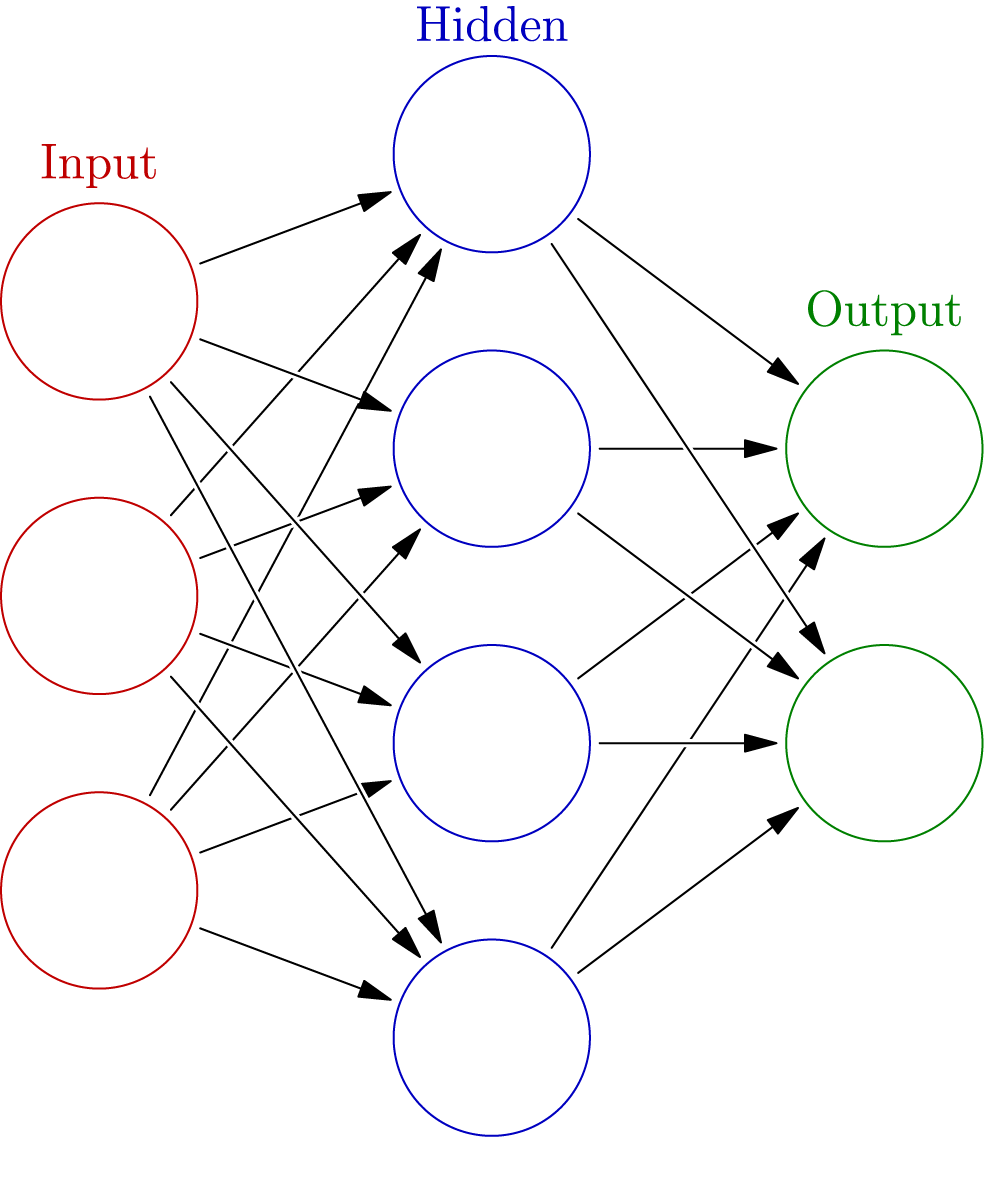
\includegraphics[width=0.50000\textwidth]{Colored_neural_network.png}

\flushleft

\url{https://commons.wikimedia.org/wiki/File:Colored_neural_network.svg}

\subsubsection{c)}\label{c}

Given a the following problems, what are sensible feedforward network
architectures (depth, width, activation function) and methods (loss
function, algorithms) that you would explore?

\begin{itemize}
\tightlist
\item
  Regression with on univariate response, 10 possible covariates, 500
  observations.
\item
  Classification with two classes, 100 possible covariates, 10000
  observations.
\item
  Classification with 10 classes, image data (like the MNIST), 50000
  observations.
\end{itemize}

\subsubsection{d)}\label{d}

What are the similarities and differences beween a feedforward neural
network with one hidden layer with \texttt{linear} activation and
\texttt{sigmoid} output (one output) and logistic regression?

\subsubsection{e )}\label{e}

In a feedforward neural network you may have \(10000\) weights to
estimate but only \(1000\) observations. How is this possible?

\subsubsection{f)}\label{f}

Which network architecture and activation functions does this formula
give?
\[ \hat{y}_1({\bf x})=\beta_{01}+\sum_{m=1}^5 \beta_{m1}\cdot \max(\alpha_{0m}+\sum_{j=1}^{10} \alpha_{jm}x_j,0)\]
How many parameters are estimated in this network?

\subsubsection{g)}\label{g}

Which network architecture and activation functions does this formula
give?

\[ \hat{y}_1({\bf x})=(1+\exp(-\beta_{01}-\sum_{m=1}^5 \beta_{m1}\max(\gamma_{0m}+\sum_{l=1}^{10} \gamma_{lm}\max(\sum_{j=1}^{4}\alpha_{jl}x_j,0),0))^{-1}\]

How many parameters are estimated in this network?

\subsubsection{h)}\label{h}

In a regression setting: Consider

\begin{itemize}
\tightlist
\item
  a sum of non-linear functions of each covariate in Module 7
\item
  a sum of many non-linear functions of sums of covariates in
  feedforward neural networks (one hidden layer, non-linear activation
  in hidden layer) in Module 11.
\end{itemize}

Explain how these two ways of thinking differ? Pros and cons?

\subsubsection{i)}\label{i}

What is the most interesting aspect of neural network (your opinion)?
How would you compare how feedforward neural networks are fitted as
compared to fitting multiple linear regression and logistic regression?
Compare how model selection (which covariates) are performed.

\section{Practical exercises}\label{practical-exercises}

You should be able to

\begin{itemize}
\tightlist
\item
  Fit regression
\item
  Fit classification with two classes
\item
  Fit classifiation with more than two classes
\end{itemize}

all with the \texttt{nnet} package. Below is an example for
classifiation with more than two classes, and a small part with
\texttt{keras} is added for completeness.

\subsection{Problem 2: Handwritten digit recognition
data}\label{problem-2-handwritten-digit-recognition-data}

See Friedman, Hastie, and Tibshirani (2001) Section 11.7.

\paragraph{Description:}\label{description}

(direct quote from \texttt{?zip.train} in \texttt{ElemStatLearn} R
package)

Normalized handwritten digits, automatically scanned from envelopes by
the U.S. Postal Service. The original scanned digits are binary and of
different sizes and orientations; the images here have been deslanted
and size normalized, resulting in 16 x 16 grayscale images.

The data are in two gzipped files, and each line consists of the digit
id (0-9) followed by the 256 grayscale values.

There are 7291 training observations and 2007 test observations.

The test set is notoriously ``difficult'', and a 2.5 excellent. These
data were kindly made available by the neural network group at AT\&T
research labs (thanks to Yann Le Cunn).

\begin{center}\rule{0.5\linewidth}{\linethickness}\end{center}

\paragraph{A selection of some images}\label{a-selection-of-some-images}

\begin{Shaded}
\begin{Highlighting}[]
\KeywordTok{library}\NormalTok{(ElemStatLearn)}
\CommentTok{# code from help(zip.train)}
\NormalTok{findRows <-}\StringTok{ }\ControlFlowTok{function}\NormalTok{(zip, n) \{}
    \CommentTok{# Find n (random) rows with zip representing 0,1,2,...,9}
\NormalTok{    res <-}\StringTok{ }\KeywordTok{vector}\NormalTok{(}\DataTypeTok{length =} \DecValTok{10}\NormalTok{, }\DataTypeTok{mode =} \StringTok{"list"}\NormalTok{)}
    \KeywordTok{names}\NormalTok{(res) <-}\StringTok{ }\DecValTok{0}\OperatorTok{:}\DecValTok{9}
\NormalTok{    ind <-}\StringTok{ }\NormalTok{zip[, }\DecValTok{1}\NormalTok{]}
    \ControlFlowTok{for}\NormalTok{ (j }\ControlFlowTok{in} \DecValTok{0}\OperatorTok{:}\DecValTok{9}\NormalTok{) \{}
\NormalTok{        res[[j }\OperatorTok{+}\StringTok{ }\DecValTok{1}\NormalTok{]] <-}\StringTok{ }\KeywordTok{sample}\NormalTok{(}\KeywordTok{which}\NormalTok{(ind }\OperatorTok{==}\StringTok{ }\NormalTok{j), n)}
\NormalTok{    \}}
    \KeywordTok{return}\NormalTok{(res)}
\NormalTok{\}}
\NormalTok{digits <-}\StringTok{ }\KeywordTok{vector}\NormalTok{(}\DataTypeTok{length =} \DecValTok{10}\NormalTok{, }\DataTypeTok{mode =} \StringTok{"list"}\NormalTok{)}
\KeywordTok{names}\NormalTok{(digits) <-}\StringTok{ }\DecValTok{0}\OperatorTok{:}\DecValTok{9}
\NormalTok{rows <-}\StringTok{ }\KeywordTok{findRows}\NormalTok{(zip.train, }\DecValTok{6}\NormalTok{)}
\ControlFlowTok{for}\NormalTok{ (j }\ControlFlowTok{in} \DecValTok{0}\OperatorTok{:}\DecValTok{9}\NormalTok{) \{}
\NormalTok{    digits[[j }\OperatorTok{+}\StringTok{ }\DecValTok{1}\NormalTok{]] <-}\StringTok{ }\KeywordTok{do.call}\NormalTok{(}\StringTok{"cbind"}\NormalTok{, }\KeywordTok{lapply}\NormalTok{(}\KeywordTok{as.list}\NormalTok{(rows[[j }\OperatorTok{+}\StringTok{ }\DecValTok{1}\NormalTok{]]), }
        \ControlFlowTok{function}\NormalTok{(x) }\KeywordTok{zip2image}\NormalTok{(zip.train, x)))}
\NormalTok{\}}
\NormalTok{im <-}\StringTok{ }\KeywordTok{do.call}\NormalTok{(}\StringTok{"rbind"}\NormalTok{, digits)}
\KeywordTok{image}\NormalTok{(im, }\DataTypeTok{col =} \KeywordTok{gray}\NormalTok{(}\DecValTok{256}\OperatorTok{:}\DecValTok{0}\OperatorTok{/}\DecValTok{256}\NormalTok{), }\DataTypeTok{zlim =} \KeywordTok{c}\NormalTok{(}\DecValTok{0}\NormalTok{, }\DecValTok{1}\NormalTok{), }\DataTypeTok{xlab =} \StringTok{""}\NormalTok{, }\DataTypeTok{ylab =} \StringTok{""}\NormalTok{)}
\end{Highlighting}
\end{Shaded}

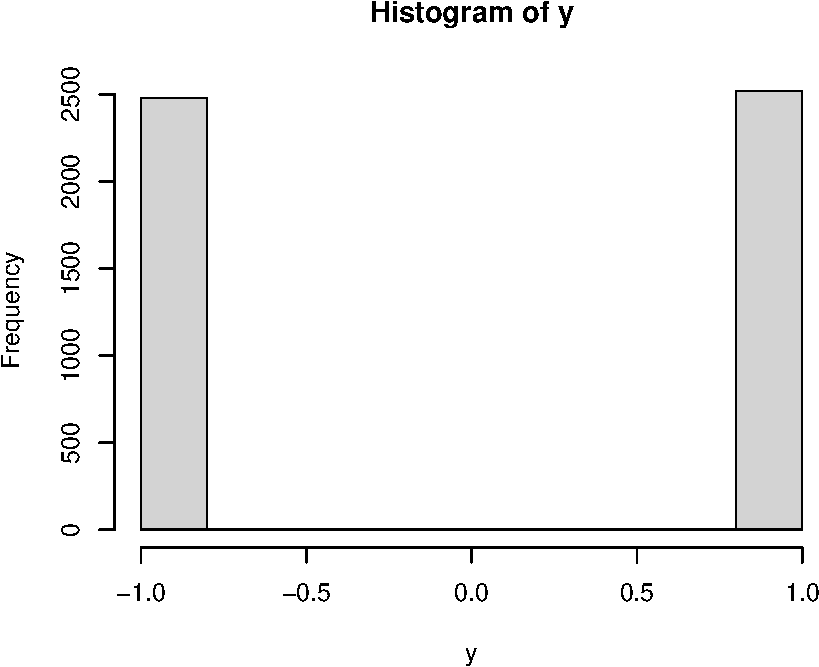
\includegraphics{RecEx11_files/figure-latex/unnamed-chunk-1-1.pdf}

\begin{center}\rule{0.5\linewidth}{\linethickness}\end{center}

\paragraph{Preprocessing data -
scaling}\label{preprocessing-data---scaling}

Important to decide on the scale based on the training data, and then
apply to both training and test data.

\begin{Shaded}
\begin{Highlighting}[]
\NormalTok{train_data =}\StringTok{ }\NormalTok{zip.train[, }\DecValTok{-1}\NormalTok{]}
\NormalTok{train_labels =}\StringTok{ }\KeywordTok{factor}\NormalTok{(zip.train[, }\DecValTok{1}\NormalTok{])}
\NormalTok{test_data =}\StringTok{ }\NormalTok{zip.test[, }\DecValTok{-1}\NormalTok{]}
\NormalTok{test_labels =}\StringTok{ }\KeywordTok{factor}\NormalTok{(zip.test[, }\DecValTok{1}\NormalTok{])}
\NormalTok{mean <-}\StringTok{ }\KeywordTok{apply}\NormalTok{(train_data, }\DecValTok{2}\NormalTok{, mean)}
\NormalTok{std <-}\StringTok{ }\KeywordTok{apply}\NormalTok{(train_data, }\DecValTok{2}\NormalTok{, sd)}
\NormalTok{train_data <-}\StringTok{ }\KeywordTok{scale}\NormalTok{(train_data, }\DataTypeTok{center =}\NormalTok{ mean, }\DataTypeTok{scale =}\NormalTok{ std)}
\NormalTok{test_data <-}\StringTok{ }\KeywordTok{scale}\NormalTok{(test_data, }\DataTypeTok{center =}\NormalTok{ mean, }\DataTypeTok{scale =}\NormalTok{ std)}
\end{Highlighting}
\end{Shaded}

\begin{center}\rule{0.5\linewidth}{\linethickness}\end{center}

\paragraph{Check out 5 hidden nodes}\label{check-out-5-hidden-nodes}

5 hidden nodes: \(257*5+6*10\)=\texttt{257*5+6*10} parameters

\begin{Shaded}
\begin{Highlighting}[]
\KeywordTok{library}\NormalTok{(nnet)}
\NormalTok{zipnnet5 <-}\StringTok{ }\KeywordTok{nnet}\NormalTok{(train_labels }\OperatorTok{~}\StringTok{ }\NormalTok{., }\DataTypeTok{data =}\NormalTok{ train_data, }\DataTypeTok{size =} \DecValTok{5}\NormalTok{, }\DataTypeTok{MaxNWts =} \DecValTok{3000}\NormalTok{, }
    \DataTypeTok{maxit =} \DecValTok{5000}\NormalTok{)}
\KeywordTok{summary}\NormalTok{(zipnnet5)}
\NormalTok{pred =}\StringTok{ }\KeywordTok{predict}\NormalTok{(zipnnet5, }\DataTypeTok{newdata =}\NormalTok{ test_data, }\DataTypeTok{type =} \StringTok{"class"}\NormalTok{)}
\KeywordTok{library}\NormalTok{(caret)}
\KeywordTok{confusionMatrix}\NormalTok{(}\KeywordTok{factor}\NormalTok{(pred), test_labels)}
\end{Highlighting}
\end{Shaded}

\begin{center}\rule{0.5\linewidth}{\linethickness}\end{center}

The above took some time to run, the results were:

\begin{Shaded}
\begin{Highlighting}[]
\OperatorTok{>}\StringTok{ }\NormalTok{zipnnet5<-}\StringTok{ }\KeywordTok{nnet}\NormalTok{(train_labels}\OperatorTok{~}\NormalTok{., }\DataTypeTok{data=}\NormalTok{train_data,}\DataTypeTok{size=}\DecValTok{5}\NormalTok{,}\DataTypeTok{MaxNWts=}\DecValTok{3000}\NormalTok{,}\DataTypeTok{maxit=}\DecValTok{5000}\NormalTok{)}
\NormalTok{iter2960 value }\FloatTok{864.566658}
\NormalTok{final  value }\FloatTok{864.561810} 
\NormalTok{converged}
\OperatorTok{>}\StringTok{ }\KeywordTok{summary}\NormalTok{(zipnnet5)}
\NormalTok{a }\DecValTok{256-5-10}\NormalTok{ network with }\DecValTok{1345}\NormalTok{ weights}
\NormalTok{options were }\OperatorTok{-}\StringTok{ }\NormalTok{softmax modelling }
\NormalTok{   b->h1   i1->h1   i2->h1   i3->h1   i4->h1   i5->h1   i6->h1   i7->h1   i8->h1   i9->h1  i10->h1  i11->h1  i12->h1  i13->h1  i14->h1  i15->h1  i16->h1  i17->h1  i18->h1 }
  \FloatTok{-49.27}     \FloatTok{9.15}     \FloatTok{1.24}    \FloatTok{21.03}    \FloatTok{-2.82}    \FloatTok{17.97}     \FloatTok{4.63}    \FloatTok{11.60}    \FloatTok{-4.31}     \FloatTok{2.28}    \FloatTok{-4.57}    \FloatTok{-6.89}    \FloatTok{-8.19}     \FloatTok{1.94}   \FloatTok{-27.05}    \FloatTok{-0.83}    \FloatTok{-8.40}   \FloatTok{-13.40}    \FloatTok{-8.07} 
\NormalTok{ i19->h1  i20->h1  i21->h1  i22->h1  i23->h1  i24->h1  i25->h1  i26->h1  i27->h1  i28->h1  i29->h1  i30->h1  i31->h1  i32->h1  i33->h1  i34->h1  i35->h1  i36->h1  i37->h1 }
\OperatorTok{>}\StringTok{ }\KeywordTok{confusionMatrix}\NormalTok{(}\KeywordTok{factor}\NormalTok{(pred),test_labels)}
\NormalTok{Confusion Matrix and Statistics}

\NormalTok{          Reference}
\NormalTok{Prediction   }\DecValTok{0}   \DecValTok{1}   \DecValTok{2}   \DecValTok{3}   \DecValTok{4}   \DecValTok{5}   \DecValTok{6}   \DecValTok{7}   \DecValTok{8}   \DecValTok{9}
         \DecValTok{0} \DecValTok{324}   \DecValTok{0}   \DecValTok{6}   \DecValTok{5}   \DecValTok{3}   \DecValTok{9}   \DecValTok{7}   \DecValTok{0}   \DecValTok{3}   \DecValTok{0}
         \DecValTok{1}   \DecValTok{1} \DecValTok{245}   \DecValTok{7}   \DecValTok{0}   \DecValTok{1}   \DecValTok{0}   \DecValTok{0}   \DecValTok{0}   \DecValTok{7}   \DecValTok{5}
         \DecValTok{2}   \DecValTok{4}   \DecValTok{7} \DecValTok{148}   \DecValTok{8}  \DecValTok{12}   \DecValTok{5}  \DecValTok{11}   \DecValTok{0}   \DecValTok{3}   \DecValTok{0}
         \DecValTok{3}   \DecValTok{2}   \DecValTok{0}   \DecValTok{6} \DecValTok{128}   \DecValTok{4}  \DecValTok{10}   \DecValTok{0}   \DecValTok{4}   \DecValTok{5}   \DecValTok{3}
         \DecValTok{4}   \DecValTok{4}   \DecValTok{1}   \DecValTok{4}   \DecValTok{0} \DecValTok{152}   \DecValTok{1}   \DecValTok{1}   \DecValTok{9}   \DecValTok{2}   \DecValTok{4}
         \DecValTok{5}   \DecValTok{1}   \DecValTok{0}   \DecValTok{2}  \DecValTok{18}   \DecValTok{1} \DecValTok{117}   \DecValTok{5}   \DecValTok{0}   \DecValTok{7}   \DecValTok{1}
         \DecValTok{6}  \DecValTok{21}   \DecValTok{3}  \DecValTok{11}   \DecValTok{0}   \DecValTok{6}   \DecValTok{1} \DecValTok{146}   \DecValTok{0}   \DecValTok{3}   \DecValTok{0}
         \DecValTok{7}   \DecValTok{0}   \DecValTok{1}   \DecValTok{6}   \DecValTok{4}   \DecValTok{5}   \DecValTok{1}   \DecValTok{0} \DecValTok{122}   \DecValTok{9}   \DecValTok{5}
         \DecValTok{8}   \DecValTok{2}   \DecValTok{2}   \DecValTok{7}   \DecValTok{3}   \DecValTok{6}  \DecValTok{15}   \DecValTok{0}   \DecValTok{1} \DecValTok{113}   \DecValTok{3}
         \DecValTok{9}   \DecValTok{0}   \DecValTok{5}   \DecValTok{1}   \DecValTok{0}  \DecValTok{10}   \DecValTok{1}   \DecValTok{0}  \DecValTok{11}  \DecValTok{14} \DecValTok{156}

\NormalTok{Overall Statistics}
                                          
\NormalTok{               Accuracy }\OperatorTok{:}\StringTok{ }\FloatTok{0.8226}          
                 \DecValTok{95}\NormalTok{% CI }\OperatorTok{:}\StringTok{ }\NormalTok{(}\FloatTok{0.8052}\NormalTok{, }\FloatTok{0.8391}\NormalTok{)}
\end{Highlighting}
\end{Shaded}

Slightly better and faster with keras, but we see that we probably need
more hidden layers since this is a difficult problem! An introduction to
\texttt{keras} is given later in this module.

\begin{Shaded}
\begin{Highlighting}[]
\KeywordTok{library}\NormalTok{(keras)}
\NormalTok{network <-}\StringTok{ }\KeywordTok{keras_model_sequential}\NormalTok{() }\OperatorTok\StringTok{ }\KeywordTok{layer_dense}\NormalTok{(}\DataTypeTok{units =} \DecValTok{5}\NormalTok{, }\DataTypeTok{activation =} \StringTok{"sigmoid"}\NormalTok{, }
    \DataTypeTok{input_shape =} \KeywordTok{c}\NormalTok{(}\DecValTok{16} \OperatorTok{*}\StringTok{ }\DecValTok{16}\NormalTok{)) }\OperatorTok\StringTok{ }\KeywordTok{layer_dense}\NormalTok{(}\DataTypeTok{units =} \DecValTok{10}\NormalTok{, }\DataTypeTok{activation =} \StringTok{"softmax"}\NormalTok{)}
\NormalTok{network }\OperatorTok\StringTok{ }\KeywordTok{compile}\NormalTok{(}\DataTypeTok{optimizer =} \StringTok{"rmsprop"}\NormalTok{, }\DataTypeTok{loss =} \StringTok{"categorical_crossentropy"}\NormalTok{, }
    \DataTypeTok{metrics =} \KeywordTok{c}\NormalTok{(}\StringTok{"accuracy"}\NormalTok{))}
\NormalTok{train_data <-}\StringTok{ }\KeywordTok{array_reshape}\NormalTok{(train_data, }\KeywordTok{c}\NormalTok{(}\DecValTok{7291}\NormalTok{, }\DecValTok{16} \OperatorTok{*}\StringTok{ }\DecValTok{16}\NormalTok{))}
\NormalTok{train_data <-}\StringTok{ }\NormalTok{train_data}\OperatorTok{/}\DecValTok{255}
\NormalTok{train_labels <-}\StringTok{ }\KeywordTok{to_categorical}\NormalTok{(train_labels)}

\NormalTok{test_data <-}\StringTok{ }\KeywordTok{array_reshape}\NormalTok{(test_data, }\KeywordTok{c}\NormalTok{(}\DecValTok{2007}\NormalTok{, }\DecValTok{16} \OperatorTok{*}\StringTok{ }\DecValTok{16}\NormalTok{))}
\NormalTok{test_data <-}\StringTok{ }\NormalTok{test_data}\OperatorTok{/}\DecValTok{255}
\NormalTok{org_test_labels <-}\StringTok{ }\NormalTok{test_labels}
\NormalTok{test_labels <-}\StringTok{ }\KeywordTok{to_categorical}\NormalTok{(test_labels)}

\NormalTok{fitted <-}\StringTok{ }\NormalTok{network }\OperatorTok\StringTok{ }\KeywordTok{fit}\NormalTok{(train_data, train_labels, }\DataTypeTok{epochs =} \DecValTok{500}\NormalTok{, }\DataTypeTok{batch_size =} \DecValTok{128}\NormalTok{, }
    \DataTypeTok{validation_split =} \FloatTok{0.2}\NormalTok{)}
\KeywordTok{library}\NormalTok{(ggplot2)}
\KeywordTok{plot}\NormalTok{(fitted) }\OperatorTok{+}\StringTok{ }\KeywordTok{ggtitle}\NormalTok{(}\StringTok{"Fitted model"}\NormalTok{)  }\CommentTok{#same as above}

\NormalTok{network }\OperatorTok\StringTok{ }\KeywordTok{evaluate}\NormalTok{(test_data, test_labels)}
\CommentTok{# acc : num 0.873}
\KeywordTok{library}\NormalTok{(caret)}
\NormalTok{res <-}\StringTok{ }\NormalTok{network }\OperatorTok\StringTok{ }\KeywordTok{predict_classes}\NormalTok{(test_data)}
\KeywordTok{confusionMatrix}\NormalTok{(}\KeywordTok{factor}\NormalTok{(}\KeywordTok{as.character}\NormalTok{(res)), org_test_labels)}
\end{Highlighting}
\end{Shaded}

\paragraph{10 hidden nodes}\label{hidden-nodes}

10 hidden nodes: \(257*10+11*10\)=\texttt{257*10+11*10} parameters

\begin{Shaded}
\begin{Highlighting}[]
\KeywordTok{library}\NormalTok{(ElemStatLearn)}
\NormalTok{train_data =}\StringTok{ }\NormalTok{zip.train[, }\DecValTok{-1}\NormalTok{]}
\NormalTok{train_labels =}\StringTok{ }\KeywordTok{factor}\NormalTok{(zip.train[, }\DecValTok{1}\NormalTok{])}
\NormalTok{test_data =}\StringTok{ }\NormalTok{zip.test[, }\DecValTok{-1}\NormalTok{]}
\NormalTok{test_labels =}\StringTok{ }\KeywordTok{factor}\NormalTok{(zip.test[, }\DecValTok{1}\NormalTok{])}
\NormalTok{mean <-}\StringTok{ }\KeywordTok{apply}\NormalTok{(train_data, }\DecValTok{2}\NormalTok{, mean)}
\NormalTok{std <-}\StringTok{ }\KeywordTok{apply}\NormalTok{(train_data, }\DecValTok{2}\NormalTok{, sd)}
\NormalTok{train_data <-}\StringTok{ }\KeywordTok{scale}\NormalTok{(train_data, }\DataTypeTok{center =}\NormalTok{ mean, }\DataTypeTok{scale =}\NormalTok{ std)}
\NormalTok{test_data <-}\StringTok{ }\KeywordTok{scale}\NormalTok{(test_data, }\DataTypeTok{center =}\NormalTok{ mean, }\DataTypeTok{scale =}\NormalTok{ std)}
\KeywordTok{library}\NormalTok{(keras)}
\NormalTok{network <-}\StringTok{ }\KeywordTok{keras_model_sequential}\NormalTok{() }\OperatorTok\StringTok{ }\KeywordTok{layer_dense}\NormalTok{(}\DataTypeTok{units =} \DecValTok{10}\NormalTok{, }\DataTypeTok{activation =} \StringTok{"sigmoid"}\NormalTok{, }
    \DataTypeTok{input_shape =} \KeywordTok{c}\NormalTok{(}\DecValTok{16} \OperatorTok{*}\StringTok{ }\DecValTok{16}\NormalTok{)) }\OperatorTok\StringTok{ }\KeywordTok{layer_dense}\NormalTok{(}\DataTypeTok{units =} \DecValTok{10}\NormalTok{, }\DataTypeTok{activation =} \StringTok{"softmax"}\NormalTok{)}
\NormalTok{network }\OperatorTok\StringTok{ }\KeywordTok{compile}\NormalTok{(}\DataTypeTok{optimizer =} \StringTok{"rmsprop"}\NormalTok{, }\DataTypeTok{loss =} \StringTok{"categorical_crossentropy"}\NormalTok{, }
    \DataTypeTok{metrics =} \KeywordTok{c}\NormalTok{(}\StringTok{"accuracy"}\NormalTok{))}
\NormalTok{train_data <-}\StringTok{ }\KeywordTok{array_reshape}\NormalTok{(train_data, }\KeywordTok{c}\NormalTok{(}\DecValTok{7291}\NormalTok{, }\DecValTok{16} \OperatorTok{*}\StringTok{ }\DecValTok{16}\NormalTok{))}
\NormalTok{train_data <-}\StringTok{ }\NormalTok{train_data}\OperatorTok{/}\DecValTok{255}
\NormalTok{train_labels <-}\StringTok{ }\KeywordTok{to_categorical}\NormalTok{(train_labels)}

\NormalTok{test_data <-}\StringTok{ }\KeywordTok{array_reshape}\NormalTok{(test_data, }\KeywordTok{c}\NormalTok{(}\DecValTok{2007}\NormalTok{, }\DecValTok{16} \OperatorTok{*}\StringTok{ }\DecValTok{16}\NormalTok{))}
\NormalTok{test_data <-}\StringTok{ }\NormalTok{test_data}\OperatorTok{/}\DecValTok{255}
\NormalTok{org_test_labels <-}\StringTok{ }\NormalTok{test_labels}
\NormalTok{test_labels <-}\StringTok{ }\KeywordTok{to_categorical}\NormalTok{(test_labels)}

\NormalTok{fitted <-}\StringTok{ }\NormalTok{network }\OperatorTok\StringTok{ }\KeywordTok{fit}\NormalTok{(train_data, train_labels, }\DataTypeTok{epochs =} \DecValTok{500}\NormalTok{, }\DataTypeTok{batch_size =} \DecValTok{128}\NormalTok{, }
    \DataTypeTok{validation_split =} \FloatTok{0.2}\NormalTok{)}
\NormalTok{allfitted <-}\StringTok{ }\NormalTok{network }\OperatorTok\StringTok{ }\KeywordTok{fit}\NormalTok{(train_data, train_labels, }\DataTypeTok{epochs =} \DecValTok{500}\NormalTok{, }
    \DataTypeTok{batch_size =} \DecValTok{128}\NormalTok{)}
\NormalTok{network }\OperatorTok\StringTok{ }\KeywordTok{evaluate}\NormalTok{(test_data, test_labels)}
\CommentTok{# acc : num 0.9133034}
\end{Highlighting}
\end{Shaded}

\section{Problem 2: Classification of diabetes cases (Compulsory problem
from
2018)}\label{problem-2-classification-of-diabetes-cases-compulsory-problem-from-2018}

During our lectures, we have used a densely connected neural network to
classify a movie review as either positive or negative using the IMDB
data set. We will use the same data here, refer to the lecture slides
for reading the data set and setting up the network.

More specifically, we have defined a linear stack of dense layers,
containing two intermediate layers containing 16 hidden units each with
reLu activation functions.

\begin{Shaded}
\begin{Highlighting}[]
\NormalTok{model <-}\StringTok{ }\KeywordTok{keras_model_sequential}\NormalTok{() }\OperatorTok\StringTok{ }\KeywordTok{layer_dense}\NormalTok{(}\DataTypeTok{units =} \DecValTok{16}\NormalTok{, }\DataTypeTok{activation =} \StringTok{"relu"}\NormalTok{, }
    \DataTypeTok{input_shape =} \KeywordTok{c}\NormalTok{(}\DecValTok{10000}\NormalTok{)) }\OperatorTok\StringTok{ }\KeywordTok{layer_dense}\NormalTok{(}\DataTypeTok{units =} \DecValTok{16}\NormalTok{, }\DataTypeTok{activation =} \StringTok{"relu"}\NormalTok{) }\OperatorTok\StringTok{ }
\StringTok{    }\KeywordTok{layer_dense}\NormalTok{(}\DataTypeTok{units =} \DecValTok{1}\NormalTok{, }\DataTypeTok{activation =} \StringTok{"sigmoid"}\NormalTok{)}
\end{Highlighting}
\end{Shaded}

Q20. What is the advantage of using a non-linear activation function
such as relu?

Q21. Why do we need to use a different activation function (sigmoid) in
the output layer instead of using relu again?

In one of our lectures, we have fitted the model above and plotted
training and validation loss as well as accuracy, as illustrated in the
figure below.

Keep two intermediate layers in the network. Try creating a simpler
model with 4 hidden units instead of 16 and a more complex model with 32
hidden units instead of 16.

Q22. Plot the training and validation loss and accuracy for the simpler
and more complex model mentioned above. How do they compare with the
model with 16 hidden units?

Q23. Besides reducing the network's size, what other methods can be used
to avoid overfitting with neural network models? Briefly describe the
intuition behind each one.

\hypertarget{refs}{}
\hypertarget{ref-ESL}{}
Friedman, Jerome, Trevor Hastie, and Robert Tibshirani. 2001. \emph{The
Elements of Statistical Learning}. Vol. 1. Springer series in statistics
New York.


\end{document}
